% -*-LaTeX-*-

\section{Evaluation}
\label{sec:eval}

% Focus on the evaluation of libpfs : is it really local speed
% Evaluation of PFSD depends on the technology that is intended to be used
% libpfs evaluation :
%    eval tech details / env
%    benchmark : LFS + small Write (relinking + meta_data updt) overhead
%    Faster than NFS_local : Definitely usable. 
%    Propagation happens asynchronously
%    without the user knowing + sequentially
% pfsd evaluation :
%    successful setup of personnal cloud
%    network usage especially on WAN still an issue
%    Hidden Costs :
%      Log size -> pruned
%      Deleted Files -> Ficus deleted files gargabe collection algorithm
% Global evaluation :
%    it's cool, but definitely not designed to scale <-> pClouds

\subsection{libpfs}

\begin{figure}[ht]
\begin{center}
  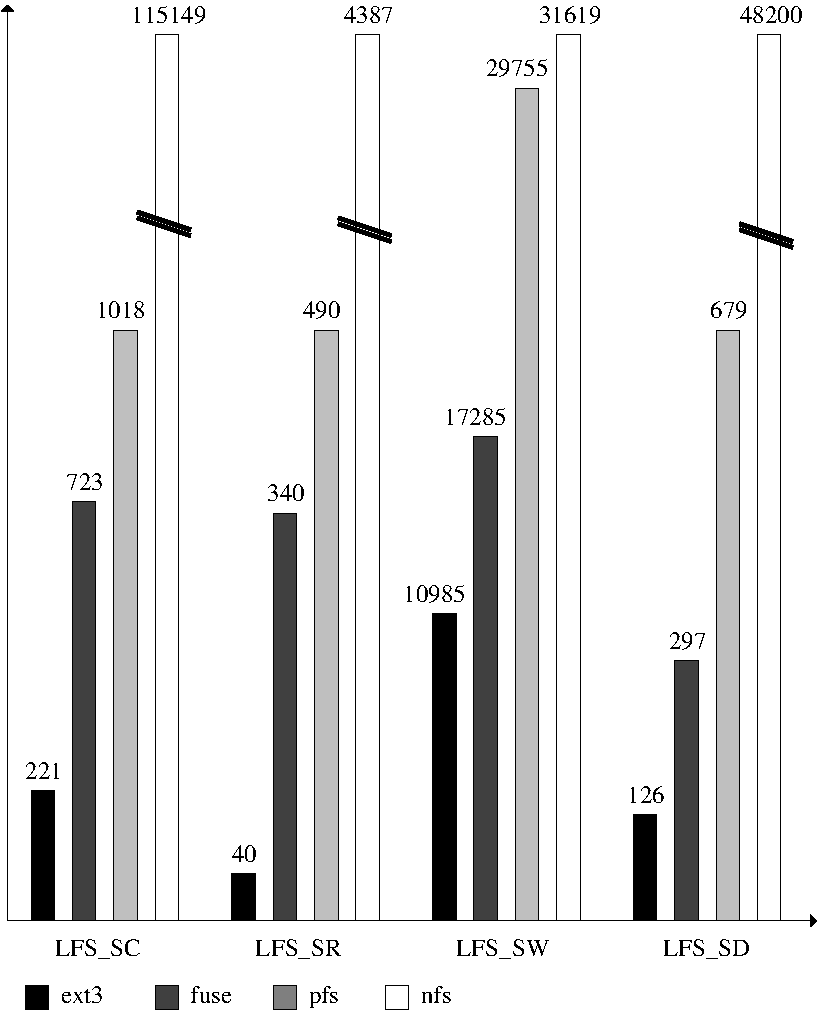
\includegraphics [scale=0.55] {fig/lfs_s}
  \caption{\label{LfsS}
    {\small LFS\_S benchmark : creation (LFS\_SC), reading (LFS\_SR),
      writing (LFS\_SW) and deletion (LFS\_SD) of 100000 small files
      in 100 directories. All values are in ms.}}
\end{center}
\end{figure}

\begin{figure}[ht]
\begin{center}
  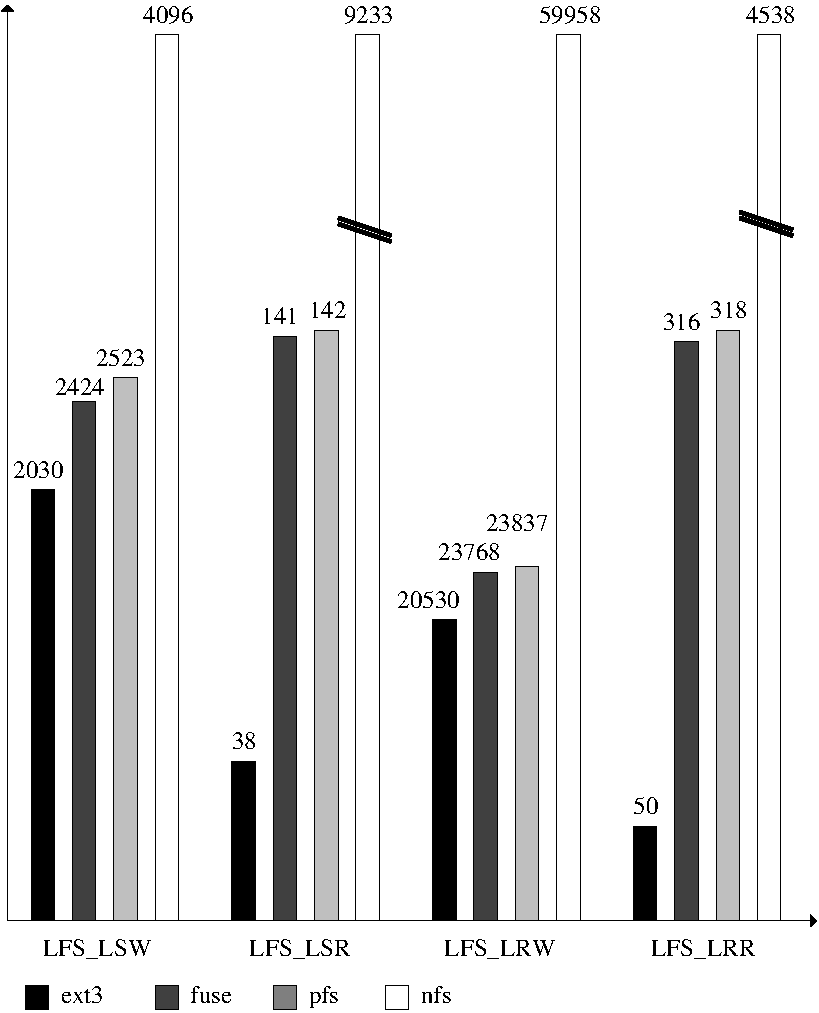
\includegraphics [scale=0.55] {fig/lfs_l}
  \caption{\label{LfsL}
    {\small LFS\_L benchmark : senquential writing (LFS\_LSW),
      sequential reading (LFS\_LSR), random writing (LFS\_LRW), random
      reading (LFS\_LRR) of a large file. All values are in ms.}}
\end{center}
\end{figure}

This section presents an evaluation of libpfs performances. Our goal is
to show that pFS provides good local performances resulting in a
seamless user experience, updates begin propagated ayncrhonously. We
compare the performances of pFS, ext3, Fuse only (We implemented a
trivial Fuse based file system replicating all calls directly to the
local file system), and NFS (Protocol v.3 over LAN with default
settings) over a set of microbenchmarks. The machine used is an 2.4
GHz Dual-Core Intel Xeon, with 2GB of RAM and a Gibabit ethernet
controller, running Ubuntu Server 8.04 distribution. The
microbenchmarks we used are the ones used for the evaluation of
LFS~\cite{rosenblum:lfs}. The small file benchmark (LFS\_S, Figure
\ref{LfsS}) consists of the creation of 100000 small (4096 bytes)
files (LFS\_SC) in 100 different directories, the access for reading
of those files (LFS\_SR), and finally their deletion (LFS\_SD). We
augmented the small file benchmark with a small file write benchmark
(LFS\_SW), which opens for writing and append a few bytes to the set
of files in order to expose the case where libpfs incurs the most
overhead (mainly, an extra {\tt link} call), as described in section
\ref{sec:impl}. The large file benchmark (LFS\_L, Firgure \ref{LfsL})
consists of writing sequentially 30000 blocks of 4096 bytes
(LFS\_LSW), reading them sequentially (LFS\_LSR), re-writing them
randomly (LFS\_LRW) and finally re-reading them randomly (LFS\_LRR).

The benchmarks are synthetic, and do not represent realistic
workloads. The goal is to show the strengths and weakness of
libpfs. Figure \ref{LfsL} shows, as expected, that versioning
maintenance does not incur any overhead compared to Fuse for large
files. pFS is substantially faster than NFS on every benchmark except
the small write benchmark (Figure \ref{LfsS}). This benchmark
emphasize the operation that incurs the most overhead due to
versionning maintenance : pFS performs comparatively to NFS on this
benchmark where it is three times slower than native ext3.

\subsection{pfsd}

Even if our prototype of pfsd is not yet optimized for bandwitdth
consumption, it already allowed us to experience the benefits of our
serverless personal cloud model. WAN and LAN communications over IP
being achieved at virtually no cost, prot\_pfsd opportunistically
communicates updates resulting in an efficient propagation of the
state among the devices. pFS is transparent to use, does not require
any maintenance once the devices are configured, and conflicts rarely
occur on a relatively well connected set of devices. We believe that
it would be really difficult to create conflicts if cell phones and
media player were to be used, even with a small capacity and a simple
LRU cache for updates. In the context of other types of communication
links, such as bluetooth on mobile devices, power consumption would
have to be considered to avoid wasting batteries.

\subsection{Hidden Costs}

There is a few hidden costs associated with the use of pFS. First, the
update log used by pfsd : even if they are deleted once propagated to
every devices, this log may grow considerably should a device remain
unused for a long period of time without being removed of the
system. ``Rumor Mongering'' technique as described
in~\cite{demers:epidemic} could be used to alleviate this issue.

Second, libpfs keeps track of deleted files to avoid ambiguity
in face of resources creation and removal. Such deleted entries are
only kept for directories that are still accessible in a group
filesystem which limits their number. Nevertheless, such entries can
be garbage collected. A solution has already been provided
in~\cite{page:ficus} under the section : ``Insert/Delete ambiguity''.

\endinput


% Local Variables:
% tex-main-file: "main.ltx"
% tex-command: "make;:"
% tex-dvi-view-command: "make preview;:"
% End:
